\documentclass[12pt]{article}

\usepackage[english]{babel}
\usepackage[utf8]{inputenc}
\usepackage{fancyhdr}

\usepackage[margin=1in]{geometry}
\usepackage{pgf}
\usepackage{pgfplots}
\usepackage{siunitx}
\usepackage{tikz}
\usepackage{float}
\usepackage{amsmath}
\usepackage{enumitem}

\usepackage[font=small,labelfont=bf]{caption}
\usepackage{pstricks-add}
\usepackage{pgfplotstable}
\usepackage[nodisplayskipstretch]{setspace}
\usepackage{hyperref}

\usetikzlibrary{scopes}
\usetikzlibrary{angles,quotes}
\usetikzlibrary{calc}
\pgfplotsset{compat=1.5}
\graphicspath{ {/} }

\newcommand*{\I}{\imath}
\newcommand*{\J}{\jmath}
\newcommand{\norm}[1]{\lvert #1 \rvert}

\setlist[enumerate, 1]{label=\alph*.}

\begin{document}
\sisetup{per-mode=symbol}

\begin{titlepage}
    \begin{center}
        \vspace*{1cm}
        \textbf{Electric Circuits}

        \vspace{0.5cm}
        Lab: 01

        \vspace{1cm}

        \textbf{Jaden Moore}

        \vfill

        Orange Coast College\\
        Engineering Circuits A285\\
        November 17th, 2021

    \end{center}
\end{titlepage}

\pagestyle{fancy}
\fancyhf{}
\setlength{\headheight}{15pt}
\lhead{Electric Circuits}
\rhead{Lab: 01}
\cfoot{\thepage}

\section{Introduction}
In this lab, we utilize DC circuit theory to analyze the voltages and currents at various nodes and elements and then compare our analysis to computer-aided design (CAD) circuit software to obtain a percent error between the two. In this case, we are utilizing the online circuit simulator CircuitLab\textregistered\space to compare with our theoretical circuit analysis.

\section{Circuit 1 Analysis and Discussion}

\begin{figure}[H]
    \begin{center}
        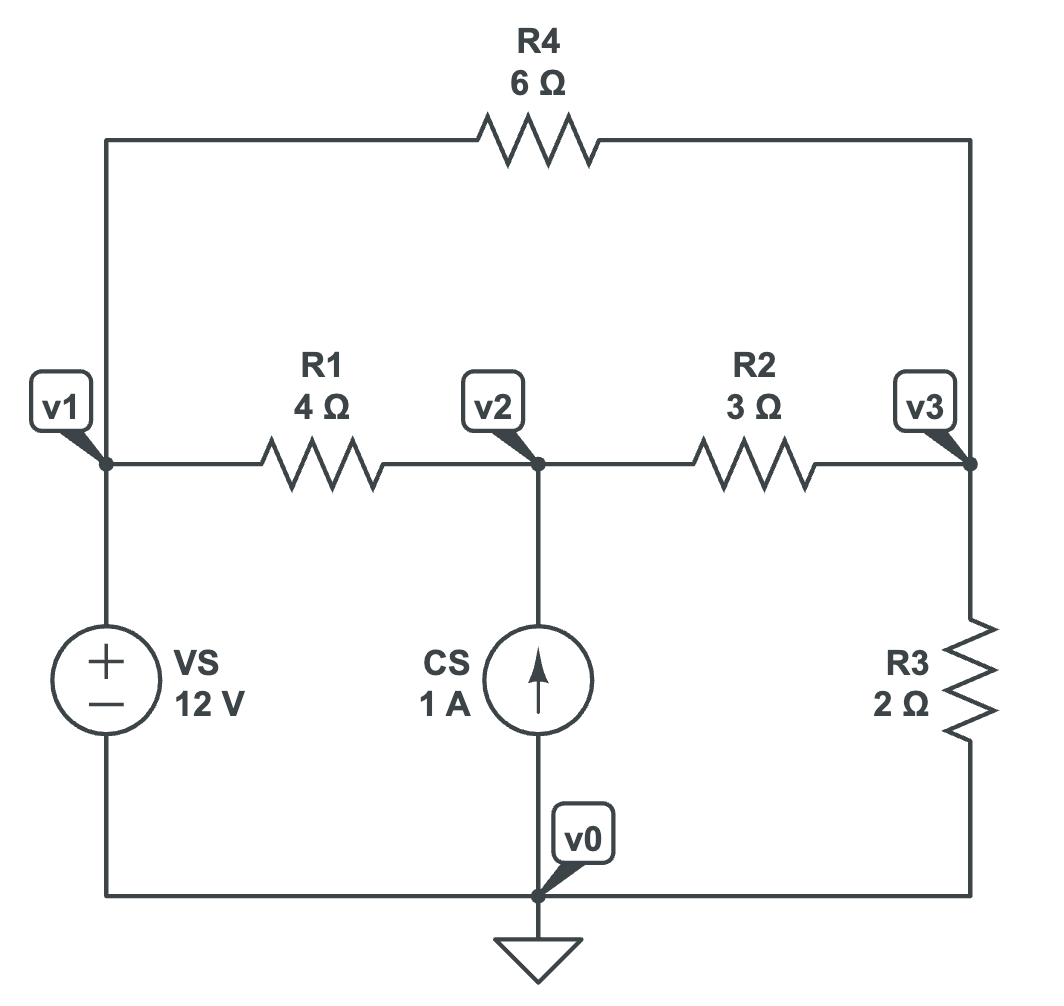
\includegraphics[scale=0.6]{circuit-1.png}
        \caption { (a) Circuit 1}
    \end{center}
\end{figure}

Consider the voltages at the specified nodes in Figure (1). We can apply nodal analysis at each node in Figure (1) to determine the voltages and then utilize CircuitLab to simulate the circuit and confirm our results.

(b) Following the path $ v_0 \rightarrow v_s \rightarrow v_1$, we see that 

\begin{equation}
    \begin{split}
        v_1 = \SI{12}{\volt}
    \end{split}
\end{equation}

\pagebreak

Applying Kirchhoff's current law (KCL) to $v_2$, we get

\begin{equation}
    \begin{split}
        &\frac{v_2 - 12}{4} + \frac{v_2 - v_3}{3} - 1 = 0 \\ 
        &7v_2 - 4v_3 = 48
    \end{split}
\end{equation}

Applying KCL to node $v_3$ we get

\begin{equation}
    \begin{split}
         &\frac{v_3 - v_2}{3} + \frac{v_3 - 12}{6} + \frac{v_3}{2} = 0 \\
         &-4v_2 + 12v_3 = 24
    \end{split}
\end{equation}

Solving Equation (2) in terms of $v_3$ and substituting it into Equation (1) we get

\begin{equation}
    \begin{split}
         &7v_2 - 4\left(\frac{24+4v_2}{12}\right) = 48 \\
         &v_2 = \SI{9.882353}{\volt}
    \end{split}
\end{equation}

Substituting $v_2$ into Equation (2) we get

\begin{equation}
    \begin{split}
        &-4(9.882353) + 12v_3 = 24 \\
        &v_3 = \SI{5.294117}{\volt}
    \end{split}
\end{equation}

(b) Using the node voltages, We can calculate the current through any branch using Ohm's Law. Thus, from theory, the current through each resistor can be calculated such that

\begin{equation}
    \begin{split}
        i_1 &= \frac{v_1 - v_2}{R_1} = \frac{12 - 9.882353}{4} = \SI{529.411}{\milli\ampere} \\
        i_2 &= \frac{v_2 - v_3}{R_2} = \frac{9.882353 - 5.294117}{3} = \SI{1.529412}{\ampere} \\
        i_3 &= \frac{v_3 - v_0}{R_3} = \frac{5.294117 - 0}{2} = \SI{2.647058}{\ampere} \\
        i_4 &= \frac{v_1 - v_3}{R_4} = \frac{12 - 5.294117}{6} = \SI{1.117647}{\ampere}
    \end{split}
\end{equation}

\pagebreak

\subsection{Circuit 1 Simulation}
Below is the values produced by the CAD simulation
\begin{figure}[H]
    \begin{center}
        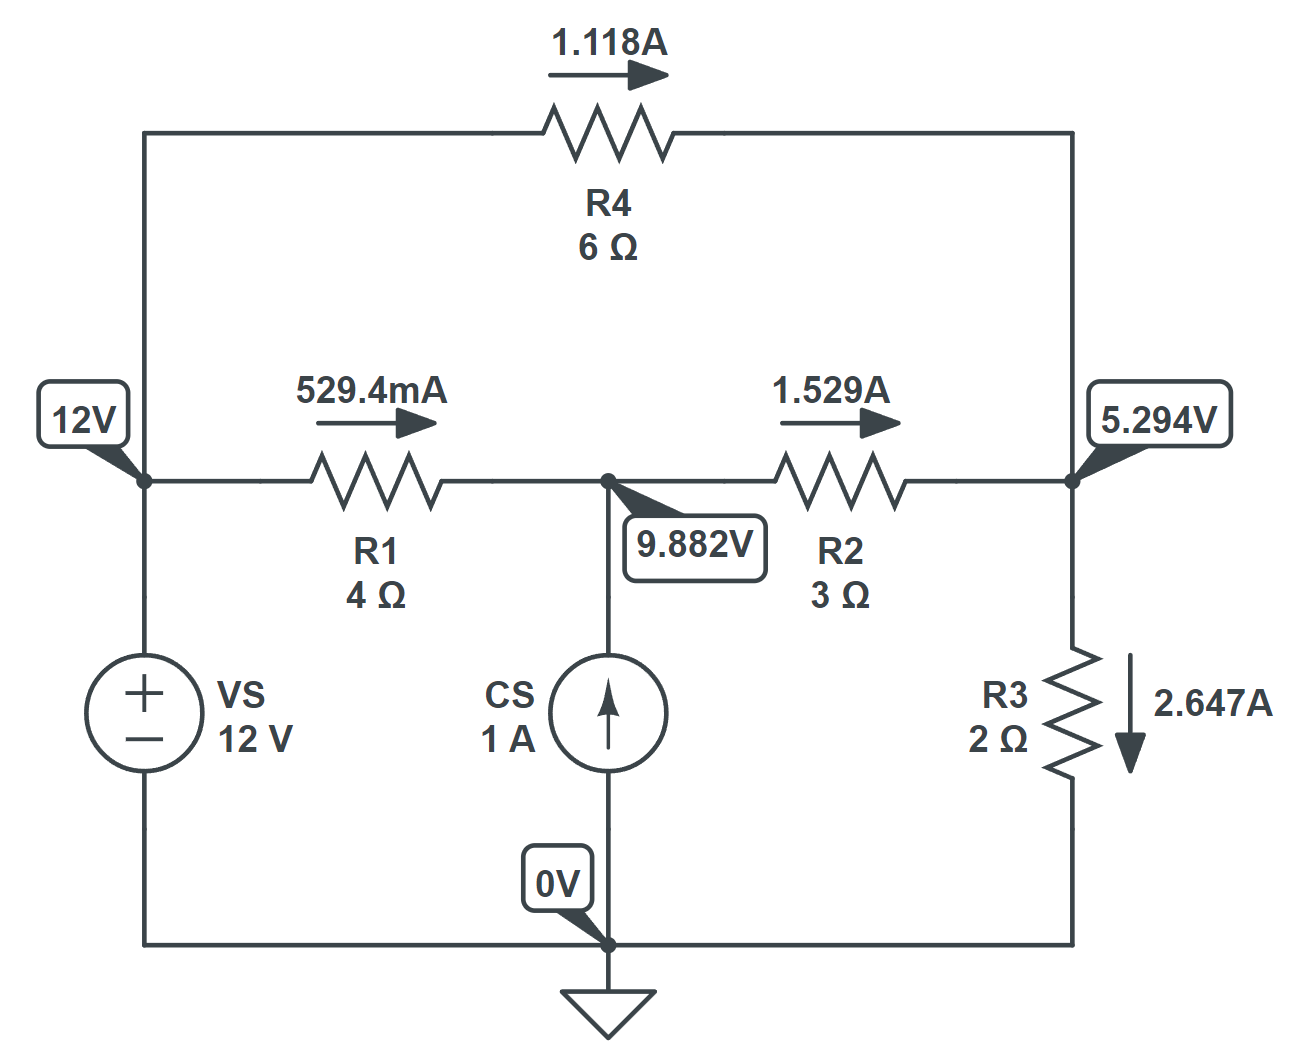
\includegraphics[scale=0.6]{circuit-1-sol.png}
        \caption { Circuit 1 CAD Simulation Results}
    \end{center}
\end{figure}

In this case, we see that the simulation produced the same currents and voltages as calculated by theory within 4 significant figures which confirms our method was accurate. We can calculate the percent error such that

\begin{equation}
    \begin{split}
        \text{\% error} &= \left( \frac{|i_{exp} - i_{theory}|}{i_{theory}} \right) 100 \\
    \end{split}
\end{equation}

As an example, we can calculate the \% error between the simulation and theory for the current $i_4$ using Equation (7) such that

\begin{equation*}
    \begin{split}
        \text{\% error} &= \left( \frac{|1.118 - 1.117647|}{1.117647} \right) 100 = 0.0315 \% \\
    \end{split}
\end{equation*}

Calculating the percent error for all current and node voltages yields a percent error of within 0.05\% which indicates the simulation was a success. Furthermore, in assessing the direction of the currents, we realize that they are flowing all flowing from a higher node potential to a lower potential which is consistent with current theory.

\section{Circuit 2 Analysis and Discussion}
\begin{figure}[H]
    \begin{center}
        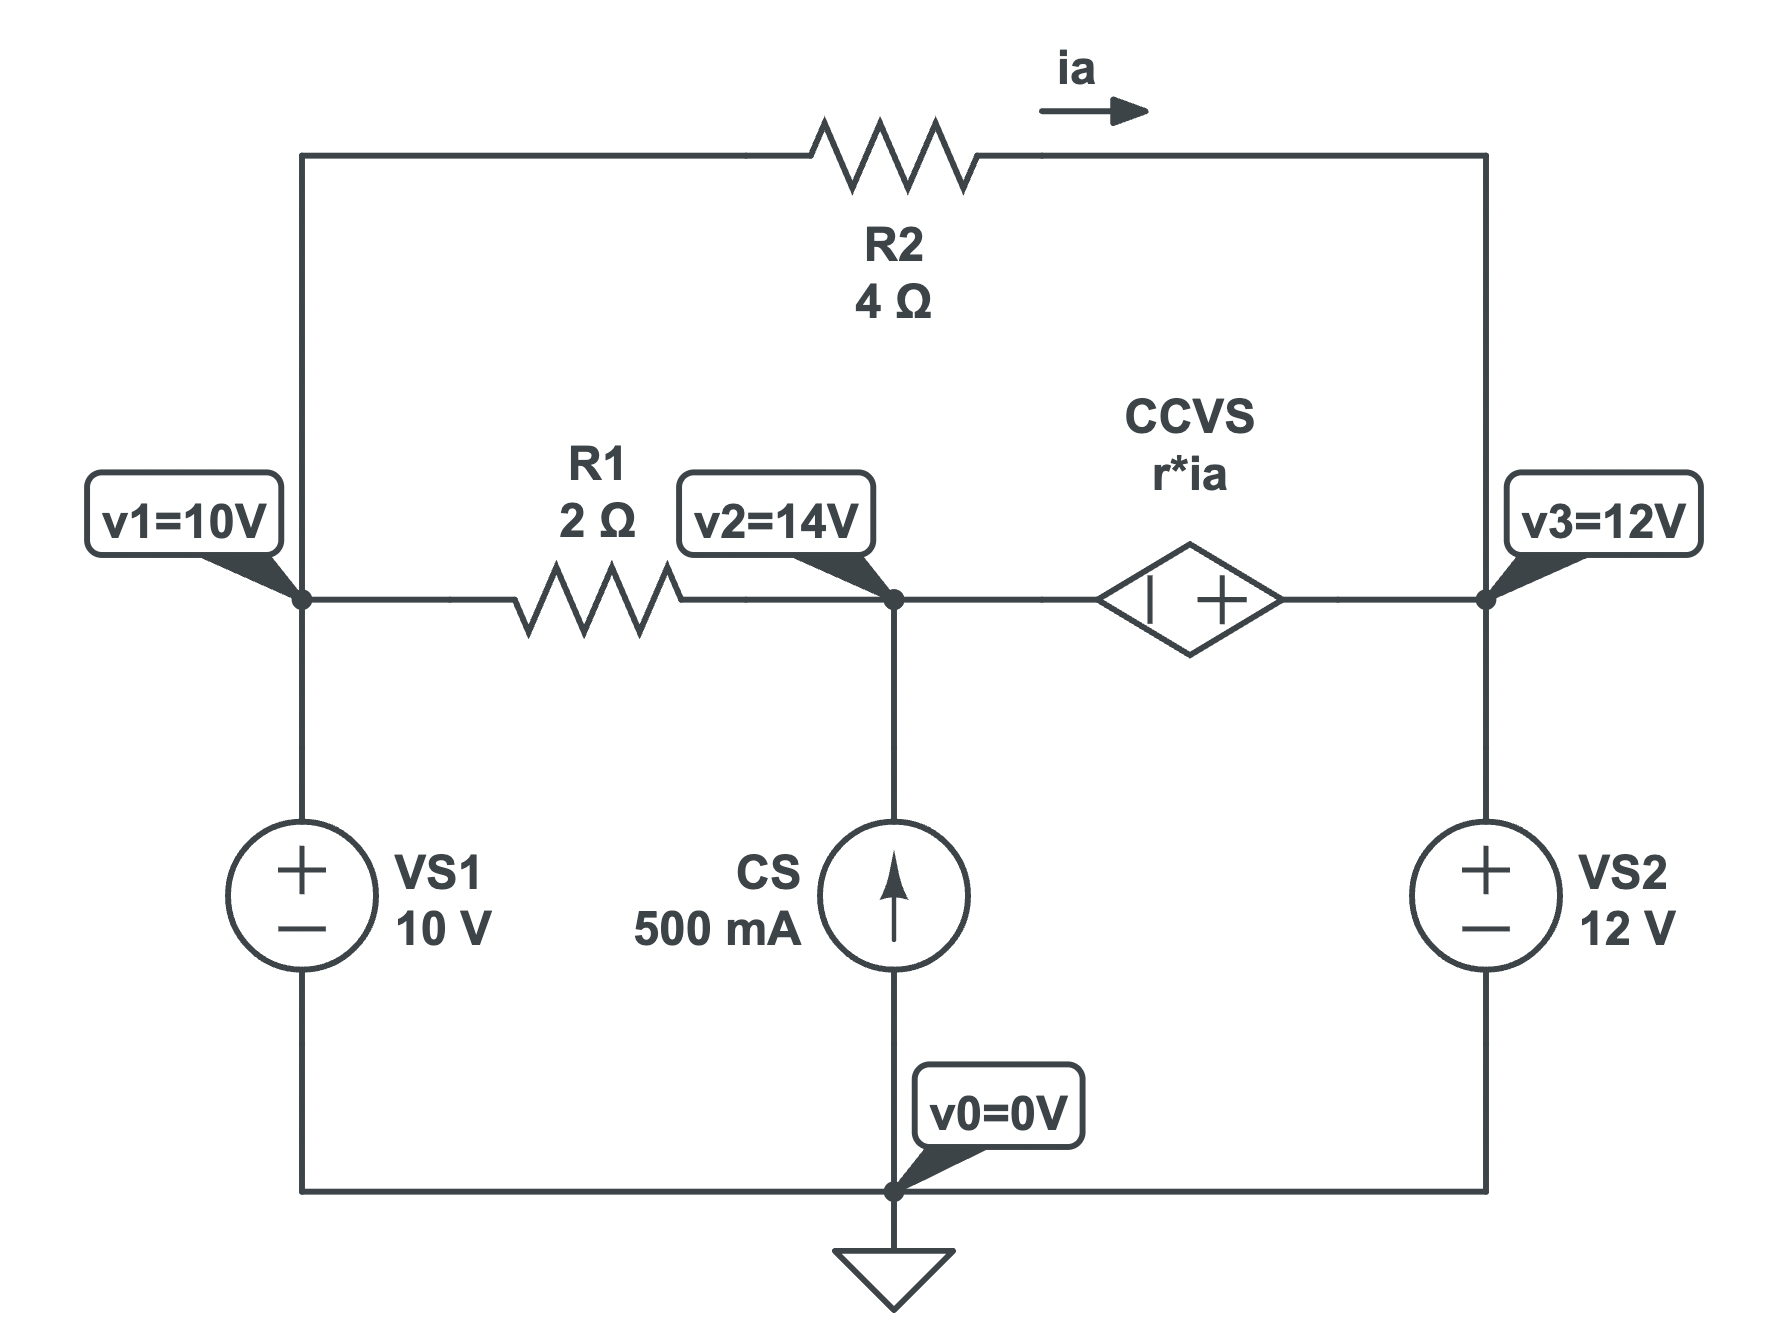
\includegraphics[scale=0.4]{circuit-2.png}
        \caption { (a) Circuit 2}
    \end{center}
\end{figure}

(b) Using theory, we can calculate the gain of the CCVS by considering the values of the voltage at nodes $v_2$ and $v_3$. That is, we can express the relationship between the CCVS its adjacent nodes by the expression

\begin{equation}
    \begin{split}
        ri_a = v_3 - v_2
    \end{split}
\end{equation}

However, $i_a$ can be expressed using Ohm's Law such that

\begin{equation}
    \begin{split}
        &i_a = \frac{v_1-v_3}{R_2} = \frac{10 - 12}{4} \\
        &i_a = \SI{-0.5}{\ampere}
    \end{split}
\end{equation}

Thus, substituting Equation (9) into Equation (8), we get

\begin{equation}
    \begin{split}
        &r(-0.5) = 12 - 14 \\
        &r = \SI{4}{V/A}
    \end{split}
\end{equation}

(c) From theory, if we instead let $v_2 = \SI{16}{V}$, we can quickly calculate the new gain of the CCVS

\begin{equation}
    \begin{split}
        &r(-0.5) = 12 - 16 \\
        &r = \SI{8}{V/A}
    \end{split}
\end{equation}

\subsection{Circuit 2 Simulation}

(d) However, in order to consider this circuit in the simulation, we must experimentally try different values for the gain until we obtain the voltage of $v_2$ that we are looking for since the simulation requires a value for the gain in order to simulate the circuit. It is clear that the voltages at $v_1$ and $v_3$ are controlled by voltage sources, thus they will never change. Thus, the CCVS directly controls the value of $v_2$ alone.

In order to test this experimentally, we tried different values of the gain until $v_2 = \SI{14}{V}$. That is we tried $r = 1, 2, 3, 4 \text{ V/A}$. Below is the circuit from the simulation

\begin{figure}[H]
    \begin{center}
        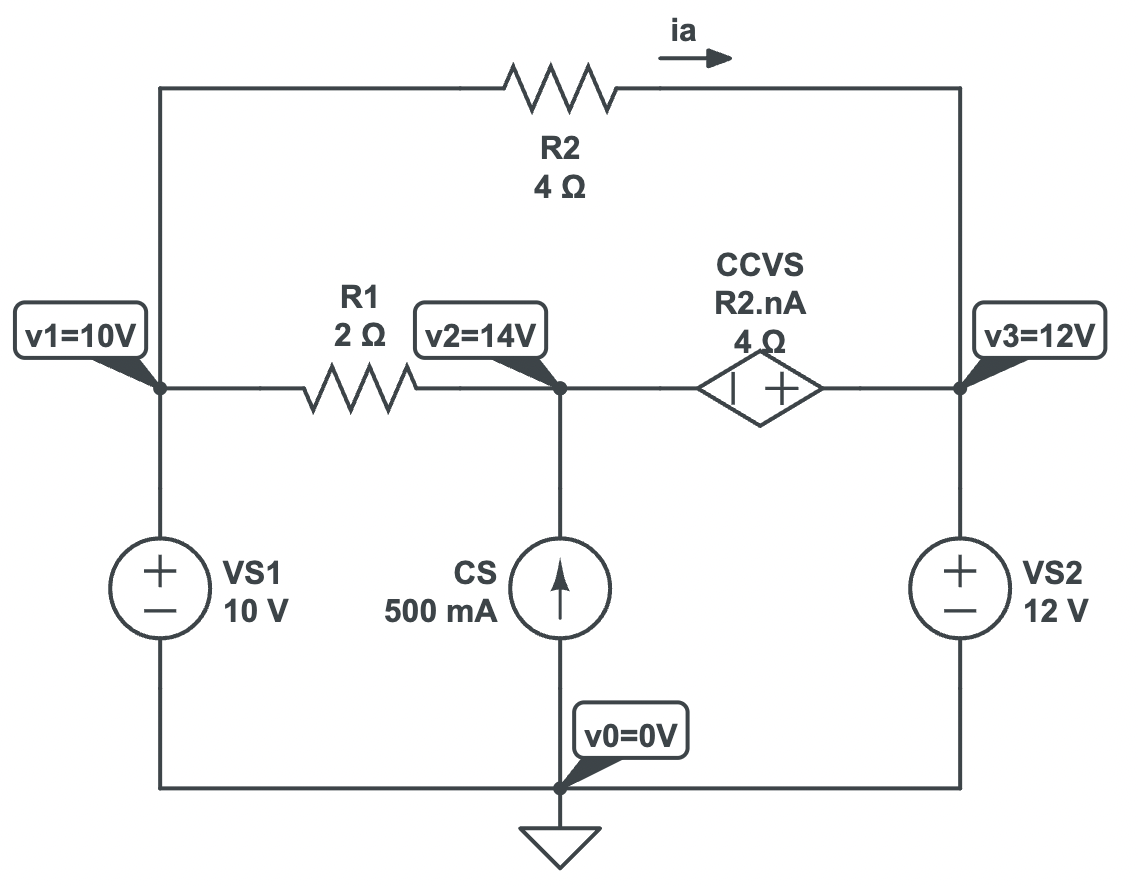
\includegraphics[scale=0.5]{circuit-2-sol.png}
        \caption { Circuit 2 CAD Simulation Results}
    \end{center}
\end{figure}


When $r = \SI{4}{V/A}$ we found that $v_2 = \SI{14}{V}$ which is consistent with our theory. We then tried increasing the value of the gain until $v_2 = 16V$. In this case, we found $v_2 = 16V$ when $r = \SI{8}{V/A}$. Thus, the result of trying different values of the gain $r$ in the simulation enabled us to find the necessary node voltage at $v_2$. We also note the \% error as calculated in Equation (7) is essentially 0\% between the experimental and theoretical value. In general, we see that every time we increase the gain $r$ by 4 V/A, the voltage at $v_2$ increases by 2V.

\section{Circuit 3 Analysis and Discussion}

\begin{figure}[H]
    \begin{center}
        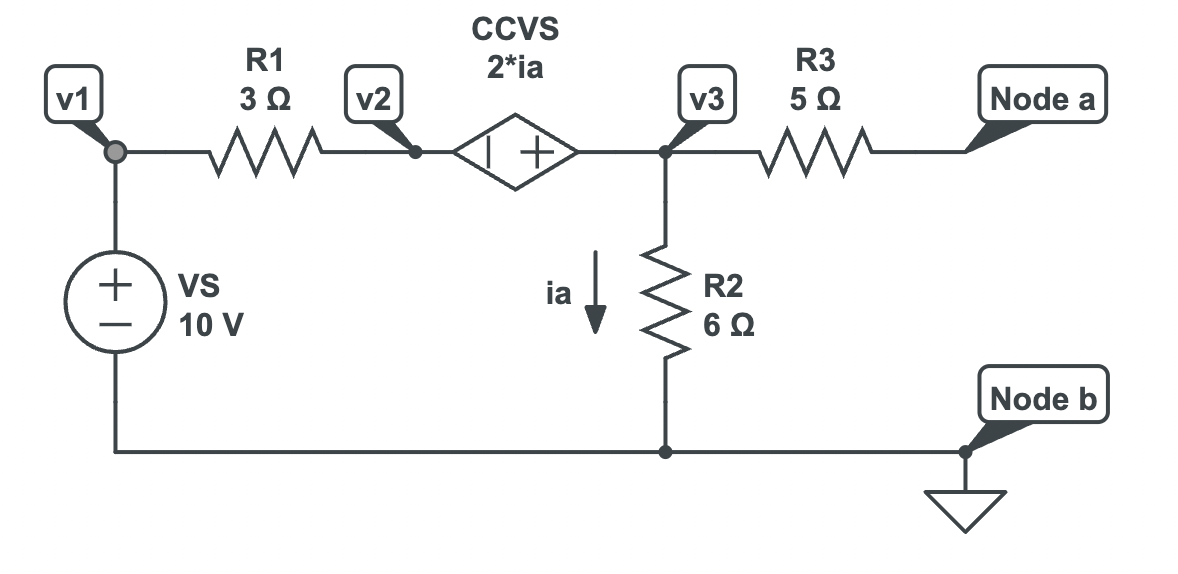
\includegraphics[scale=0.6]{circuit-3.png}
        \caption { (a) Circuit 3}
    \end{center}
\end{figure}

In order to analyze this circuit, we will first convert it to Thévenin's equivalent circuit with respect to terminals a-b. The first thing we note is that the voltage across $R2$ is equal to the voltage across terminals a-b. That is,

\begin{equation*}
    \begin{split}
        v_3 - 0 = v_{oc} 
    \end{split}
\end{equation*}

Therefore, we can apply the nodal analysis method to determine the voltage across $v_{R2}$. First, we see $v_1 = 10V$ due to $V_s$. Then we apply KCL at $v_3$.

\begin{equation}
    \begin{split}
        &\frac{v_3}{6} + \frac{v2-10}{3} + 0 = 0 \\
        &v_3 + 2v_2 = 20
    \end{split}
\end{equation}

From inspection, we see that

\begin{equation}
    \begin{split}
        &v_2 = v_3 - 2i_a \\
        &v_2 = v_3 - 2\left(\frac{v_3}{6}\right)
    \end{split}
\end{equation}

Substituting Equation(13) into Equation (12), we get that

\begin{equation}
    \begin{split}
        &v_3 + 2v_2 = 20 \\
        &v_3 + 2\left(v_3 - 2\left(\frac{v_3}{6}\right)\right) = 20 \\
        &v_3 = v_{oc} = \SI{8.5714}{V}
    \end{split}
\end{equation}

We can then apply a short circuit across terminals a-b in Figure (5) to obtain $i_{sc}$. In this case, we can apply nodal analysis to $v_3$ to obtain the current through terminals a-b.

\begin{equation}
    \begin{split}
        &\frac{v_3}{6} + \frac{v2-10}{3} + \frac{v_3}{5} = 0 \\
        &11v_3 + 10v_2 = 100
    \end{split}
\end{equation}

Substituting Equation(13) into Equation (15), we get that

\begin{equation}
    \begin{split}
        &11v_3 + 10\left(v_3 - 2\left(\frac{v_3}{6}\right)\right) = 100 \\
        &v_3 = \SI{5.6603}{V}
    \end{split}
\end{equation}

Thus, we can calculate $i_{sc}$ such that

\begin{equation}
    \begin{split}
        &i_{sc} = \frac{v_3}{R3} = \frac{5.6603}{5} \\
        &i_{sc} = \SI{1.13207}{\ampere}
    \end{split}
\end{equation}

After obtaining $v_{oc}$ and $i_{sc}$, we can then calculate $R_{th}$ such that

\begin{equation}
    \begin{split}
        &R_{th} = \frac{v_{oc}}{i_{sc}} = \frac{8.5714}{1.13207} \\
        &R_{th} = \SI{7.5714}{\ohm}
    \end{split}
\end{equation}

Below, we redraw Figure (5) into Thévenin's equivalent circuit.

\begin{figure}[H]
    \begin{center}
        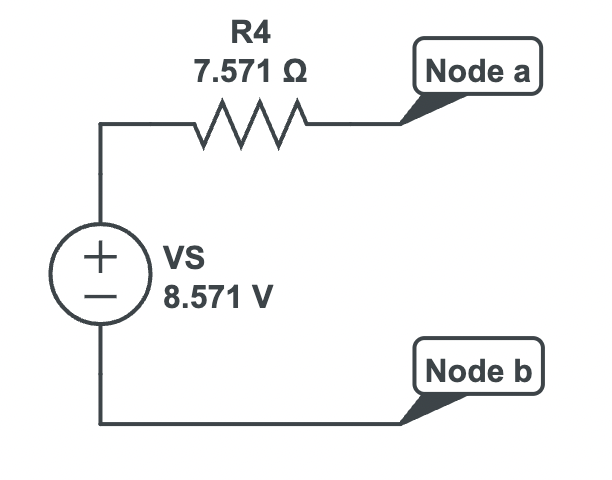
\includegraphics[scale=0.6]{circuit-3-v2.png}
        \caption { (b) Thévenin's equivalent of Figure (5) }
    \end{center}
\end{figure}

\subsection{Circuit 3 Simulation}
Below we draw the Figure (5) which the values obtained from the simulation.

\begin{figure}[H]
    \begin{center}
        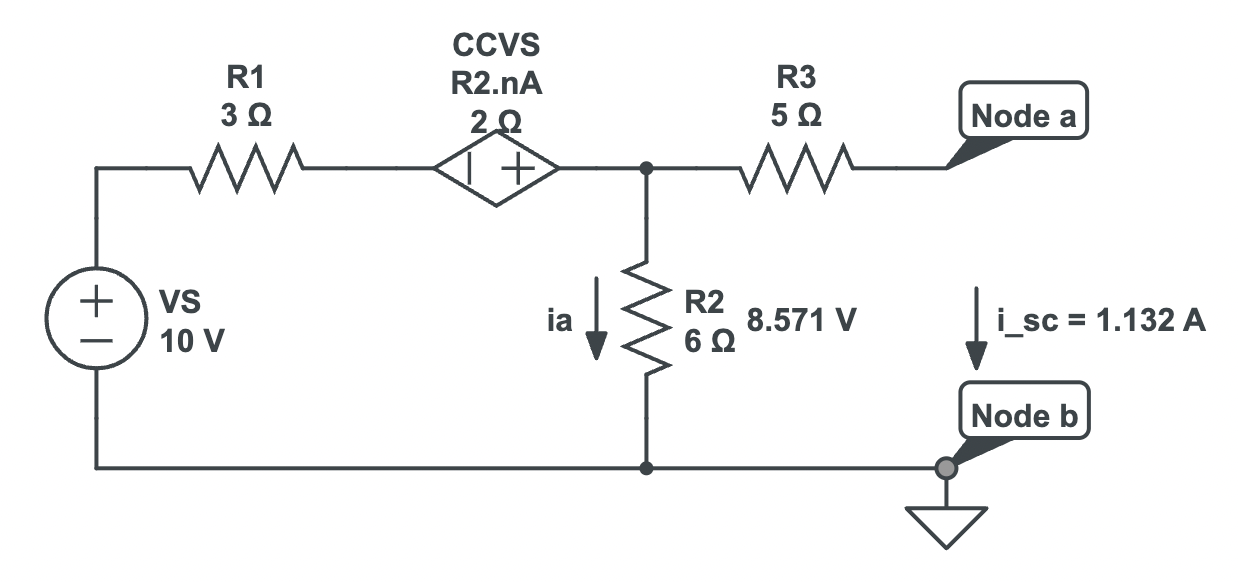
\includegraphics[scale=0.6]{circuit-3-sol.png}
        \caption { (c) CAD Simulation of Circuit 3 }
    \end{center}
\end{figure}

(d) In order to find Thévenin's equivalent circuit using CircuitLab, we simply examine the voltage at Node a in the simulation. Thus, we quickly get

\begin{equation}
    \begin{split}
        &V_{oc} = v_a = \SI{8.571}{V} \\
    \end{split}
\end{equation}

We then attach a wire across terminals a-b in the simulation to obtain a current through it. In this case we get that

\begin{equation}
    \begin{split}
        &i_{sc} = \SI{1.132}{A}
    \end{split}
\end{equation}

The process to find Thévenin's equivalent circuit from the simulation requires creating two versions of the circuit, one without a wire across a-b and one with a wire. Then, the analysis becomes very straightforward. Following the process in Equation (18), we get Thévenin's equivalent circuit from the simulation to be the same as Figure (6) from theory. In this case, using Equation (7) to calculate the percent error, we get a 0\% error with respect to the experimental and theoretical values.

\pagebreak

\section{General Discussion and Conclusion}
In general, we get that circuit simulations using CircuitLab are consistent with circuit theory up to 4 significant figures. After 4 significant figures, the simulation rounds, which loses some accuracy compared to theory. However, every result from theory and simulation was within 0.05\% error with respect to each other. One important aspect of simulating the circuits was ensuring the correct orientation of the resistor elements such that the current is flowing into the positive terminal. This was critical to ensure, otherwise we were getting incorrect results. Another critical aspect was ensuring that we connected the current controlled voltage sources to the correct current, otherwise the CCVS produces the incorrect voltage.

We also conclude that the values obtained in both theory and the simulation are reasonable because the values of the input voltage sources and voltage gains are within the possibility of producing the currents and voltages obtained in each circuit. Our analysis included the combination of Ohm's Law, Kirchhoff's Laws, and Thévenin's Theorem. One can find the in-depth analysis within each circuit section in the lab.

We also note that in the analysis of real circuitry, we would encounter much more significant margins of error with respect to theory. Potential sources of this error are most commonly in the non-ideal nature of wire, faults and resistance in voltage sources, as well as potentially different resistances than expected in resistor elements that can occur in real world applications.

\pagebreak

\section{CircuitLab Reference}
All experimentation was done using the online web-based circuit builder, CircuitLab which is found here: \url{https://www.circuitlab.com/}. There are no special requirements to run the software since it is browser based. In this lab, the website was utilized on Google Chrome in both Linux and Windows environments.

This tool is preferred because it requires no download or installation and allows you to create basic and more advanced circuits very quickly while still offering most of the advanced features that industry software offers. It also makes it very easy to share circuits through links instead of large files.

\begin{figure}[H]
    \begin{center}
        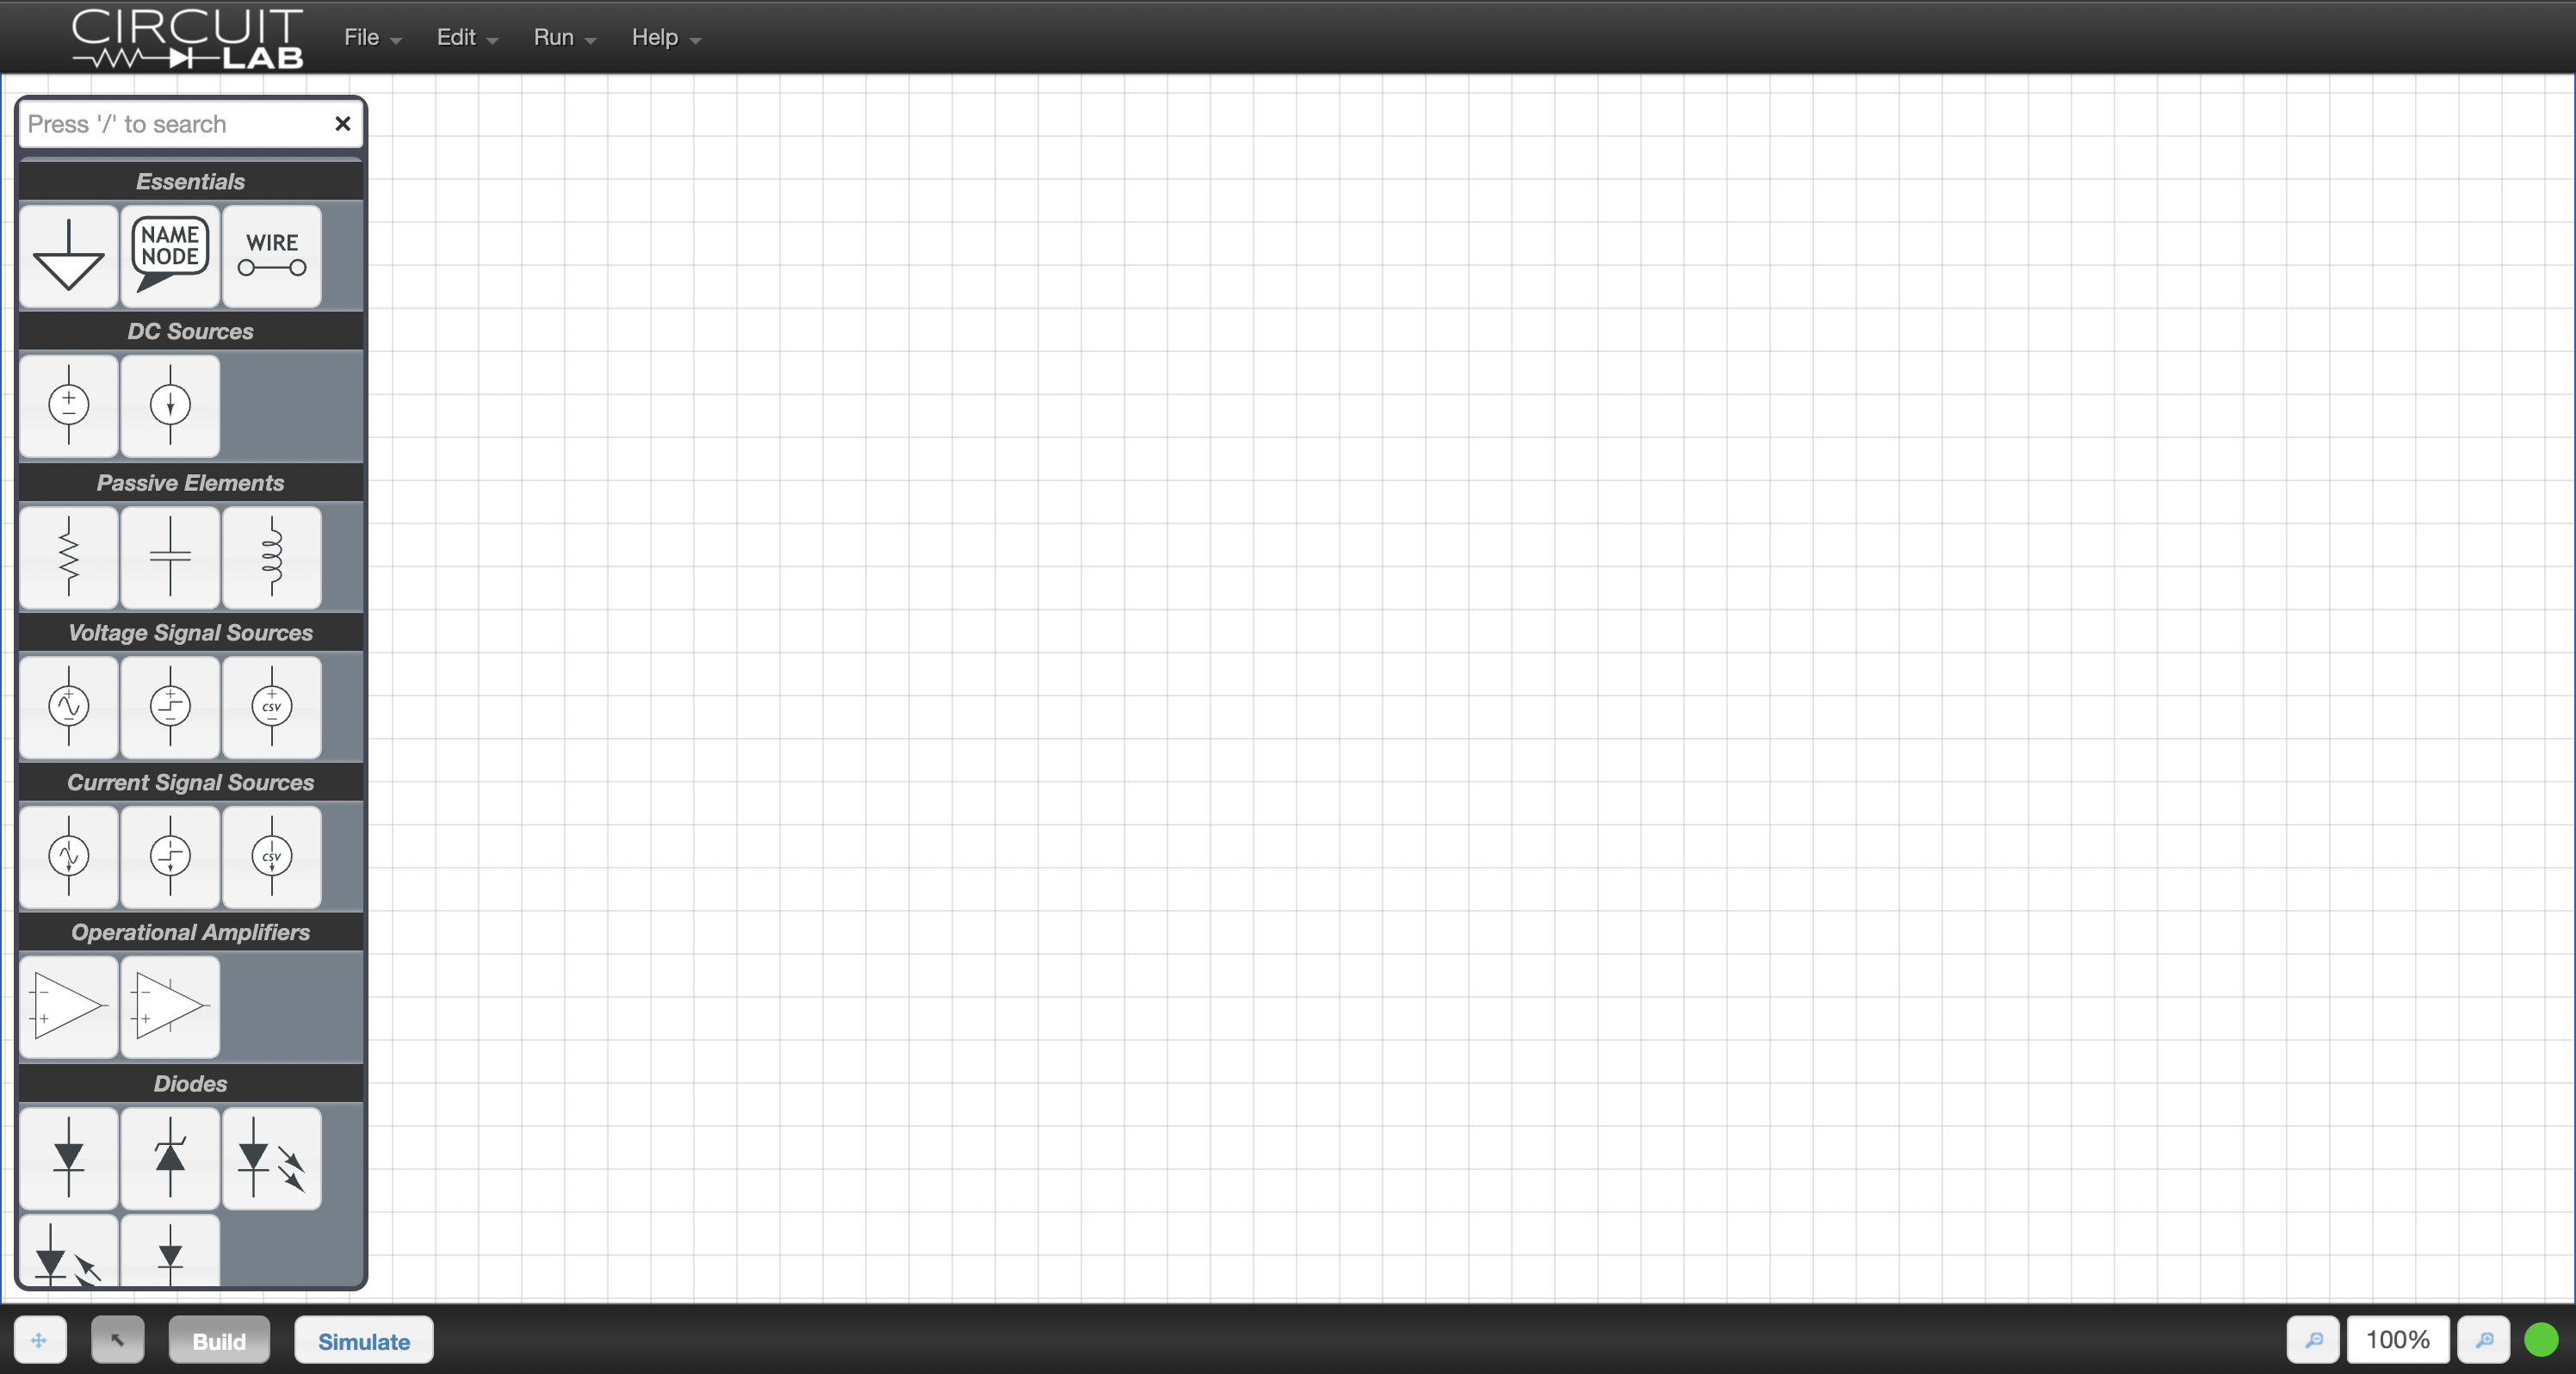
\includegraphics[scale=0.3]{circuit-lab.png}
        \caption { CircuitLab interface}
    \end{center}
\end{figure}

In comparing it to orCAD, microcap, and micro-sim, we find that it offers very similar functionality in terms of circuit elements offered, and basic time dependent voltage and current graphing. Although the aforementioned tools offer more in-depth features than CircuitLab, CircuitLab is able to handle all the functionality we need at this level of circuit analysis.
Below are the links to access each circuit referenced in this lab:

\begin{itemize}
    \item Circuit 1: \url{https://www.circuitlab.com/editor/#?id=8bxu6yasv639}
    \item Circuit 2: \url{https://www.circuitlab.com/editor/#?id=bjzg28a3q28a}
    \item Circuit 3: \url{https://www.circuitlab.com/editor/#?id=rtexy736m8qq}
  \end{itemize}

\pagebreak

\subsection{How to Simulate}
In order to simulate the circuit, you must click "Simulate" in the bottom left corner of the editor, and then under the "DC" category, you click the "Run DC Solver" button.

\begin{figure}[H]
    \begin{center}
        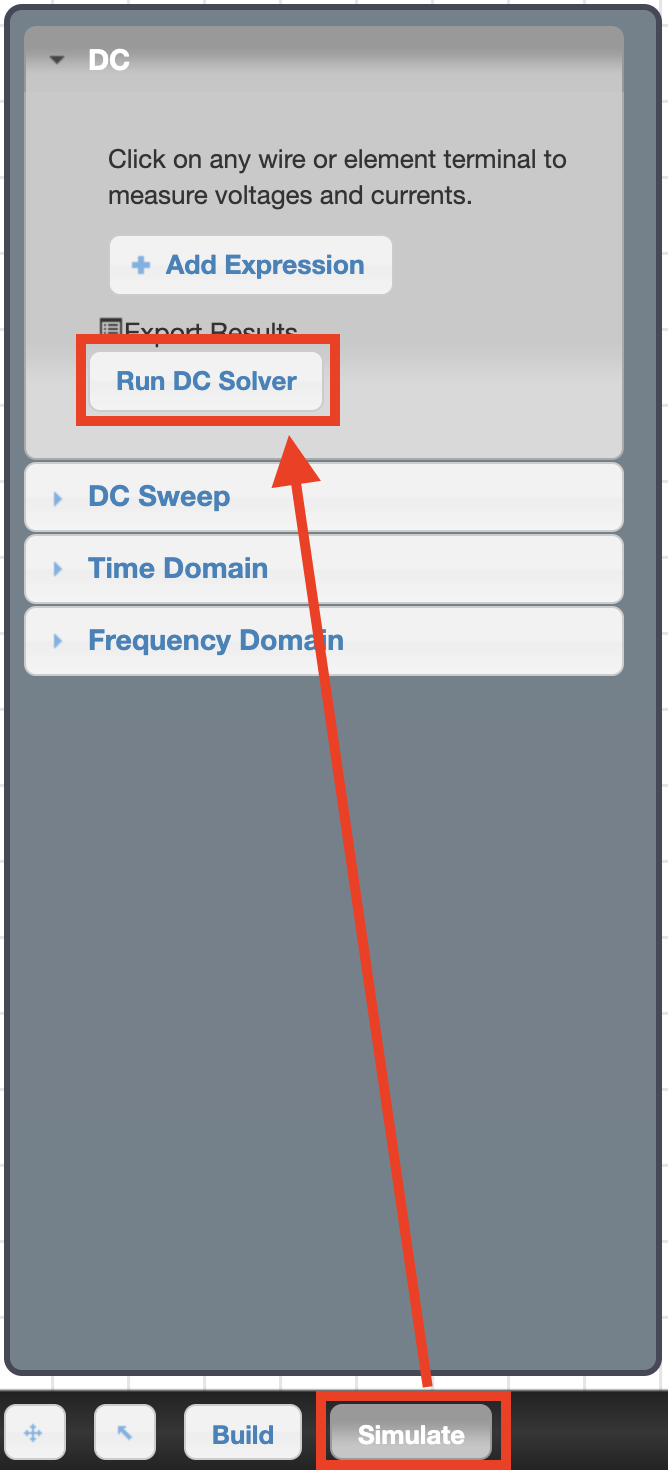
\includegraphics[scale=0.5]{circuit-lab-tut.png}
        \caption { CircuitLab Simulation Steps}
    \end{center}
\end{figure}

Once you run the DC Solver, you must switch back to build mode by clicking "build" at the bottom of Figure (9). Then, you can hover your mouse over any node or element to obtain the associated voltage and currents.
\end{document}